\documentclass[tikz, border=2pt]{standalone}

\usepackage{tikz,tikz-layers,amsmath}
\usetikzlibrary{shapes.geometric,calc,positioning}
\usepackage{xcolor}
\usepackage{fontawesome5} % For the \faUser (person) icon


\begin{document}
\begin{tikzpicture}

\node[draw, semithick, minimum width=3cm, minimum height=1.35cm, outer sep=0pt] (box) {};

\node[ circle, inner sep=0pt, minimum size=.3cm, fill=black!70] (c1) at ($(box.center)+(-1.15,.25)$) {};
\node[ circle, inner sep=0pt, minimum size=.3cm, fill=black!70] (c2) at ($(box.center)+(-1.15,-.25)$) {};

\node[minimum width=.75cm, minimum height=.8cm, right=.5cm of {$(c1)!.5!(c2)$}] (r) {};
\draw[semithick, line cap=round] 
(r.west)--(r.east) 
($(r.west)+(0,-.18)$)--($(r.east)+(0,-.18)$)
($(r.west)+(0,-.36)$)--($(r.east)+(0,-.36)$)
($(r.west)+(0,.18)$)--($(r.east)+(0,.18)$)
($(r.west)+(0,.36)$)--($(r.east)+(0,.36)$);

\node[draw, semithick, circle, inner sep=0pt, minimum size=.8cm, outer sep=0pt] (c3) at ($(box.center)+(.9,0)$) {};
\draw[semithick, line cap=round] (c3.west)--(c3.east) (c3.center)--+(0,.25);

\node[draw, semithick, minimum width=.5cm, minimum height=.75cm, outer sep=0pt, right=0cm of box] (r2) {};
\draw[semithick, line cap=round] (r2.north)--(r2.south);

\node[draw, semithick, minimum width=1cm, minimum height=.75cm, outer sep=0pt, above=0cm of box] (r3) {};
\node[minimum width=2.5cm, minimum height=.75cm, outer sep=0pt, above=0cm of r3] (r4) {\footnotesize Estimator};
\draw[semithick, line cap=round] (r3.west)--(r3.east);
\draw[semithick, line cap=round] (r3.north west)--(r4.north west)--(r4.north east)--(r3.north east);

\node[inner sep=0cm, above=1mm of r4, scale=1.9, label={above:\footnotesize Data}] {\color{black!70}\faDatabase};
% \node[right=.5cm of r2, label={above:\scriptsize Estimate}] (beta) {$\hat{\beta}$};
\node[right=.25cm of r2] (beta) {Estimate $\hat{\beta}$};

\node[ellipse, minimum width=1.5cm, minimum height=1cm, left=2cm of r, yshift=1cm, label={[yshift=1mm]above:\small Estimand}] (ell) {$\beta$};
\draw[semithick] (ell.west) to[bend left=45] (ell.north west) to[bend left=55] (ell.north) to[bend left=60] (ell.north east) to[bend left=85] (ell.east) to[bend left=55] (ell.south east) to[bend left=35] (ell.south) to[bend left=45] (ell.south west) to[bend left=35] cycle;

\node[draw, semithick, circle, inner sep=1mm] (b1) at ($(ell.south west)+(-.2,-.2)$) {};
\node[draw, semithick, circle, inner sep=.5mm, below left=1mm of b1] {};


\end{tikzpicture}
\end{document}
